\chapter[A Fine Gentleman, Inspiring Teacher and A Passionate Scientist]{Professor Gowravaram Ramachandran: A Fine Gentleman, Inspiring Teacher and A Passionate Scientist}\label{chap31}

\Authorline{H S Vinay Deepak}

The results of the entrance test for master's degree programs had been announced.
Since I had been shortlisted at a few places, I had to choose a place among them.
However, I could not imagine myself staying in a hostel and boarding in a
canteen, so I had a major problem. The thought of going out of my home city
Bangalore, for further studies always brought a feeling of discomposure.
Nevertheless, I had to make a choice very soon. So, as an attempt to overcome
my unease, I thought it would be a good idea to have a peek into hostels and
canteen by conducting a recce of universities and institutes in other cities. In one
such trip, I landed in Mysore and headed straight to the University hostel and
canteen. Unimpressed with the canteen, I headed to the department that offered
me a seat. As I explored the department's classrooms, a thought crossed my mind,
that may be, a chat with any available professor might help. The next thing I saw
on my right was a name plate, `Prof.\ G Ramachandran'. Without knocking I
slipped in to see a gentleman with a pleasing, sagely demeanor involved in
discussions with five students sitting around his table. Participants appeared
relaxed and the ambience was quite friendly. However, looking at what was
written on the board, I could sense some really highbrow theoretical physics was
being unveiled. I walked further and stood right across his table and introduced
myself and then conveyed the reason for my rather abrupt intrusion. To my
comfort, Prof.\ GR agreed `Yes, it is a good idea to know the place you want to
study'. After few minutes of conversations, I abruptly asked Prof.\ GR what he did
as research. Suddenly, I could sense the feeling of shock fill the room. Although
alarmed, he patiently and enthusiastically described what was going on in his
group and introduced me to the persons involved in it. After a while, he asked me what
made me choose physics, while he gently probed about the books that made me 
lean towards physics. Surprisingly, he took my squeamishness and discomfort of
boarding outside rather kindly and advised I may do well studying in Bangalore
University itself. However, he invited me to participate in weekly lectures on
quantum mechanics he conducted every Saturday. Thus, began a relationship
with Prof.\ GR that was to shape and affect me in more than one way.

Today, as I sit down reminiscing my interactions with Prof.\ GR, I am very much
aware how truly privileged and honored I am to write about `The Prof.\ G
Ramachandran' I knew. I am also aware how unqualified I am to write about his
distinguished career and his research accomplishments. My relationship with Prof.\ 
GR is atypical in many ways, as I was not his formal class room student working
for any degree in the institutions he worked. Ours was a relationship between two
enthusiasts. One whose passion was to teach and guide and other who loved to
hear and learn from him. At any rate, I am his proud student and GR my beloved
teacher.

After many years of knowing him, it still appears easier for me to write about
circumstances that spurred me to form the picture of Prof.\ GR as an
ideal teacher than to describe Prof.\ GR's personality. His Saturday lectures were
invariably full in capacity, with the audience consisting of many post graduate
students from his own department, doctoral research students at various stages of
their thesis and also few greenhorns like me. There were also somewhat senior
participants who worked as teachers in nearby colleges just wanting to experience
the grandeur of the subject through GR's lectures.

In his saturday lectures, he would blend the glory and drama in story of quantum
mechanics without drifting away from brass tacks and rigorous essentials of the
topic. He presented the mathematics of quantum mechanics just enough to
describe concepts with clarity rather than to make it appear needlessly grand or
pompous. This way he kept novice toddlers like me involved. He consciously
made efforts to ensure that novices like myself did not feel out of place. I never
ever saw him use written notes while he filled up the board with equations as he
lectured the class that almost always went beyond two hours. Neither did I sense
his energy diminish. His adroit statements during his lectures appeared to be read
out from his mind's book that was written very early in his career. His lectures
were always peppered with copious amounts of anecdotes and stories of
individuals who contributed immensely to physics. His exposition always aimed
at laying a strong foundation of basics and then swiftly taking students through
the later developments more often in chronological sequence. He would at some
stage begin to propose possible research projects to the class that deserved to be
explored. After the lecture, some of us would walk along to his home, for doubt
clarifications with tea and snacks served lovingly by Mrs.\ Ramachandran and
another round of discussion on research problems.

It didn't take long for me to realize that there was nothing in his personality to
suggest that Prof.\ GR would have yearned for higher positions of authority or
limelight. For him, being with students and teaching them what he knew was most
gratifying. His passion for teaching interested students went on well into his last
days. More often, I had the privilege of playing the role of organizer or event
manager for such teaching sessions whenever a handful of students gathered and
asked for it.

After my postgraduation, I felt theoretical physics was not for me. I enjoyed
tinkering with devices and substances, so took up experimental physics for my
Ph.D. at IISc. I was worried that this decision would taper off my academic
interactions with GR. However, on the contrary our relationship grew stronger.
Every time we met; he was always curious to hear what I was doing. What was
previously a `he teaches and I learn' interaction gradually evolved into `we
debate, I learn' type of interaction. During many such interactions, he would
throw new light and elucidate the topic which in turn, gave me better prespective
and clarity about what I was attempting to describe. He would always appeal that
a good theoretical grip would pay dividends as conceptual clarity and eventually
feed into novel experimental insights.

As an experimentalist I had difficulties in describing my work to Prof.\ GR,
because he always demanded I start from the interaction Hamiltonians \cite{chap31-key1}.
However, I must say I always had a great time discussing them and at the end of
it all, I was always the beneficiary. I had worked mainly on novel Nuclear
Magnetic Resonance spectroscopic methodologies applied to oriented systems.
Liquid crystals exhibit a rich variety of phases and properties. NMR spectroscopy
is a very powerful tool to study the various phases and interactions at the
microscopic level and geometrical parameters at the molecular scales \cite{chap31-key2}. It has
also turned out that some of these properties can be usefully utilized for
investigation of both small and large molecules by NMR with rich rewards for
applications and fundamental understanding.

My research involved both pure liquid crystalline materials as well as molecules
oriented in liquid crystalline matrices \cite{chap31-key3},\cite{chap31-key16}. In particular investigations related
to various aspects of NMR in liquid crystalline media, such as, assignment of
resonances, director dynamics of spinning liquid crystals in different phases and
with various symmetry, thereby leading to novel techniques to characterize the
liquid crystalline phase have been carried out. Simplified methods for structure
determination of solutes dissolved in liquid crystal solvents have been proposed.
Diffusion ordered spectroscopy of a mixture of liquid crystals of opposite
diamagnetic susceptibility at its coexistent phase was also used and studied,
besides chiral discrimination using anisotropic NMR interactions with particular
emphasis in bio-molecular applications.

NMR spectroscopy which has become a method of choice for understanding
ordering mechanisms of mesogens requires a robust method for obtaining
assignments of the NMR spectra of various nuclei that are found in the mesogens.
It turns out that the spectra in the isotropic phase and in the nematic phase of a
liquid crystal molecule are very different due to the presence of chemical shift
anisotropy in the mesophase spectrum. There are a host of methodologies
available for assigning spectra in the isotropic phase \cite{chap31-key4}. These methods, however
fail, when applied to the spectrum of the molecules in the mesophase due to the
dominating role of strong anisotropic interactions, such as homonuclear
couplings among protons. To circumvent these problems, a property of the liquid
crystal molecules under off-magic angle sample spinning can be utilized. It was
shown that the director/symmetry axis of a liquid crystal with positive
diamagnetic susceptibility anisotropy ($\Delta \chi$) aligns along the spinning axis for $\theta$
between $0^{\circ}$ and $\theta_m$, where $\theta$ is the angle between the spinning axis and the
magnetic field and $\theta_m = 54.7^{\circ}$ is the magic angle. It may be noted that the
spectrum of $\theta = 0^{\circ}$ spinning angle corresponds to the normal static spectrum,
while the spectrum of $\theta = \theta_m$ corresponds to the isotropic spectrum. In an earlier
study the ${}^{13}C$ liquid crystal spectra was recorded as a function of very closely
spaced $\theta$ values from $90^{\circ}$ all the way up to $0^{\circ}$. From these plots of chemical shift
versus the angle of spinning it is possible to follow the trajectory of each
${}^{13}C$ spectral line from its position from $\theta = \theta_m$ to $\theta = 0^\circ$ and then match the spectrum
in the isotropic phase (equivalently the magic angle sample spinning spectrum of
the nematic phase) to the spectrum of the static sample in the nematic phase.
However, this method requires recording spectra at closely spaced angle intervals
to unambiguously follow the trajectory of each of the lines without missing out
any crossover of trajectories. However, this operation is time consuming. We
proposed an alternate method, where we utilize the fact that the above trajectory
has a very distinct relationship to the isotropic and anisotropic chemical shift and
the problem of assignment does not require a continuous variation of angles, but
just a few selected experiments should enable the assignment of the spectrum in
the anisotropic phase. Thus, the method of assignment has been made simpler and
faster. It is shown that in addition to the assigned isotropic spectrum, only one
other Off-magic angle sample spinning spectrum whose spinning angle $\theta$ is
accurately known is necessary to obtain the complete assignment of the static
spectrum. This procedure is non-trivial due to possibilities of errors in
assignments, arising out of inaccuracies in the knowledge of chemical shifts and
the spinning angle. A computational procedure is proposed to take into account
deviations arising out of non-ideal experimental conditions. A discussion
regarding the details of the procedure and also situations where there can be
ambiguities and how they can be resolved has been published \cite{chap31-key5}. The developed
method has been demonstrated on a well-known thermotropic liquid crystalline
system, N-(4-ethoxybenzylidene)-4-n-butlyaniline [EBBA]. Since assignment of
resonances in the nematic phase is a primary requirement for any further analysis
regarding the ordering and deeper understanding of the role of various
substituents in the mesogens, clearly this novel prescription can be of immense
use and utility.

The study of director dynamics in a lyotropic liquid crystal composed of
Potassium laurate, 1-Decanol and $D_2 O $ \cite{chap31-key6} under variable angle sample spinning
using ${}^2$H~ NMR spectrum of $D_2~ O$ was undertaken. A very interesting interplay of
the magnetic orienting torque due to interaction of the liquid crystal director with
the magnetic field and viscous torque arising from the viscosity of the sample on
the director comes to fore. The relative magnitude of these torques has a direct
bearing on the spectral pattern and line shapes observed, providing valuable
insights into magnetohydrodynamics of the spinning liquid crystals. This study
lead to even more interesting behaviour for liquid crystals which deviate from
uniaxial symmetry. This competition between magnetic and viscous torques has
been quantitatively visualized by simulation of the ${}^2H$ spectrum. It has also been
possible to visualize the observed spread in the director distribution arising out of
viscous torque in terms of the energetics of the system under fast spinning. If the
magnetic torque dominates over the viscous torque, then the equilibrium
corresponds to the director orientation of $\delta = 0^\circ$ with respect to the spinning axis,
where the energy is at its minimum. However, the viscous and magnetic torques
can become comparable as it may happen if the spinning angle is close to the
magic angle or when the $\Delta \chi$ of the system is small \cite{chap31-key7}. In those circumstances
additional energy from the viscous torque causes the distribution of the director
orientation to spread further away from $\delta = 0^{\circ}$ for a positive $\Delta\chi$ liquid crystal.
The spectrum of the biaxial phase \cite{chap31-key8} as a function of the spinning angle shows
more interesting director distribution. Here the patterns of the director distribution
are observed on either side of the magic angle due to the presence of more than
one director. The patterns observed also have information about the symmetry of
the phase. This work provides insights into magnetohydrodynamics of spinning
liquid crystals and can also be of relevance to samples of biological interest such
as bicelles with proteins or peptides oriented in them. \cite{chap31-key9}

Subsequent Investigations also dealt with a novel characterization method
relevant for the biaxial phase. As an off shoot of the previous investigation it
effectively overcomes the disadvantages of the previous experimental methods
which require simulation and line shape fitting to extract useful parameters \cite{chap31-key10}.
We present the measurement of geometrical parameters of oriented solutes in
phases exhibiting biaxial symmetry. The measured parameters show the effect of
the onset of biaxiality as significant deviation in the value of the measured
parameter \cite{chap31-key11}.

The utility of liquid crystalline media as solvents in high resolution NMR
spectroscopy has been very rewarding since the pioneering work of Saupe and
Englert \cite{chap31-key12}. The intramolecular interactions within solutes are only partially
averaged. As a result, one obtains a liquid like spectrum while at the same time
very useful anisotropic interactions such as dipolar couplings, chemical shift
anisotropies, quadrupolar couplings and anisotropic part of spin-spin J couplings
are extracted. NMR spectra of molecules dissolved in thermotropic liquid crystals
have long been used to obtain structural and orientational information. At the
same time the complexity of the spectrum increases with the increase in the
number of spins and the reduction in symmetry of the molecule, which can make
the spectral analysis forbidding. Generally, proton spectra have been used to
obtain the geometry of the proton skeleton of the molecule and the information
that includes dilute X nuclei such as ${}^{13}C$ and ${}^{15} N$ are available only from satellites
which are buried in the relatively intense proton spectrum. Different inequivalent
dilute spins coupled to protons form different coupled spin systems in their
natural abundance and appear as satellites in the proton spectra. Identification of
transitions belonging to each of the spin system is essential to determine
heteronuclear dipolar couplings, which is a formidable task. Investigation dealing
with development of the techniques to obtain the complete structure of the
dissolved molecules including nuclei other than protons in their natural
abundance was also conducted. The use of inverse experiments was demonstrated
to overcome the problems of sensitivity and complexity for solute molecules
having larger number of spins. In studies using Heteronuclear Single Quantum
Coherence (HSQC) and Heteronuclear Multiple Quantum Coherence (HMQC)
experiments, we have selectively detected spectra of each inequivalent rare spin
coupled to protons in pyrazine, pyrimidine and pyridazine dissolved in
thermotropic Phase 4 and Phase 5 liquid crystal solvents. This way we could
obtain enhancement in the intensity of satellites signals without the interference
from the signals connected to the major isotopomers \cite{chap31-key13}-\cite{chap31-key14}. Besides, we could
resolve a complex spectrum into its sub-spectra corresponding to individual ${}^{13}C$
and ${}^{15} N$ isotopomers. This separation of the spectra corresponding to individual
sub-spin systems makes analysis easy and helps analyse larger systems with
higher number of spins and lower symmetry. Besides ${}^1 H-{}^1 H$ dipolar couplings,
${}^{13} C- {}^1 H$ and ${}^{15} N- {}^1 H$ dipolar couplings have been determined in natural abundance,
thereby giving the complete dipolar coupling network between all the spins in the
molecule. In this treatment pyrazine, pyrimidine and pyridazine have been used
as examples of methodology developed. It is expected that the method will be of
wider use for several other similar systems.

The diffusion ordered spectroscopic investigation was conducted on a phase
arising out of mixing together two liquid crystals having opposite signs of
diamagnetic susceptibility anisotropy \cite{chap31-key15}. Towards this end we have used
CH$_3$CN as a probe molecule. The spectrum of CH$_3$CN has with it the information
about the parallel or perpendicular orientation of the phase. Such a mixture of
liquid crystals have shown interesting behaviour at the critical temperature where
the two phases seem to coexist. It has been an interesting question to understand
what exactly happens for the molecular orientation when the macroscopic
anisotropy $\Delta \chi$ vanishes. Earlier the temperature was very finely varied taking due
precautions to maintain homogeneity and stability of temperature to the tune of
$\pm~ 0.05$K across the sample volume. The observation of a powder pattern exactly
in the critical temperature was interpreted as arising out of a distribution of
directors equally oriented in all directions. In our experiments we have measured
the diffusion coefficient of the probe molecule i.e. acetonitrile as we change the
temperature of the system through the critical temperature. At the critical
temperature we have a situation of being able to measure the parallel and
perpendicular orientational diffusion coefficients simultaneously. The
measurements show that the parallel component of the diffusion coefficient has
reduced and the perpendicular component has increased in comparison to the
trend in the immediate neighbouring temperatures, thereby indicating that at the
exact critical condition the liquid crystal mixture consists of an isotropic
distribution of molecules. As a check to rule out any exchange of molecules in
different domains of parallel and perpendicular orientations an Exchange
Spectroscopy (EXSY) experiment was conducted with a mixing time which was
same as that of the diffusion delay in the DOSY experiment. The EXSY spectrum
showed no exchange cross peaks between the two orientations, this confirms that
the anisotropy of the diffusion vanishes at the critical temperature \cite{chap31-key16}.

Gradually, Prof.\ GR began to get interested in experiments concerning spinning
liquid crystal. We attempted to rigorously understand the behaviour of mesogens
considering the interplay of moment of inertia and diamagnetic susceptibility
tensors. We were particularly interested if the ability to manifest a specific
director distribution could arise from a relationship between molecular shape
biaxiality with its diamagnetic susceptibility tensor. We also set out trying to
understand how molecular properties can be related to macroscopic anisotropic
properties in liquid crystals using relevant orientational order parameters.

On many occasions Prof.\ GR did prod me to work on theoretical physics. He
envisaged a line of investigation that could lead to a laboratory test for Axions
\cite{chap31-key17}. Two more friends joined the Axion group. He would give a series lecture
on Quantum electrodynamics and guide us towards the path of calculations. It
was for this work he enabled us to read one of the most famous and authoritative
book written by R P Feynman \cite{chap31-key18}. Subsequently, Prof.\ Ramnath Cowsik too
pitched in to contribute to the project. We met Prof.\ Cowsik whenever he was here
in Bangalore at RRI to discuss the direction the project was taking. Subsequent
consultations mostly took place over mail. It was evident that Prof.\ Cowsik and
Prof.\ GR shared a great deal of mutual respect, admiration and affection to each
other. Encouraging words from Prof.\ Cowsik was an energiser to youngsters like
us. Prof.\ Cowsik reminded us as to how lucky we were to learn physics and QED
from Prof.\ GR, whom he described as one of the able and best Master to learn
from. Infact, this sentiment echoed itself when I met Prof.\ ECG Sudarshan too.
Prof.\ B V Sreekantan was always highly appreciative of Prof.\ GR's untiring
passion to teach and his prolific contributions in the form of regular publications
in spite of his advanced age.

Prof.\ G R achieved what an ideal teacher would hope for, love, affection and
respect from all their students. Prof.\ GR's students will have a thousand reasons
to remember him all their life. I for one still do not know why I was bestowed
with his warmth, affection and trust. I owe Prof.\ GR an immense debt of gratitude
for everything I received. Mentored by Prof.\ GR and knowing him for so long will
remain one of the high points of both my career and life. I am sure I will continue
to be inspired by his erudition, his gracefulness and above, all his silent dignity.

\begin{thebibliography}{99}
\bibitem{chap31-key1} Principles of High Resolution NMR in Solids, M. Mehring, Springer-Verlag, 1976.

\bibitem{chap31-key2} Nuclear Magnetic Resonance of Liquid Crystals, R. Y. Dong, Springer - Verlag, 1994.

\bibitem{chap31-key3} NMR Basic principles and Progress, P. Diehl and C. L. Khetrapal, 1, Springer Verlag, Heidelberg, 1969.

\bibitem{chap31-key4} Principles of Nuclear Magnetic Resonance in One and Two Dimensions, R. R. Ernst, G. Bodenhausen and A. Wokaun, Oxford University Press, 1987.

\bibitem{chap31-key5} H. S. Vinay Deepak, Anu Joy, N. Suryaprakash and K. V. Ramanathan. Magn.\ Reson.\ Chem.\ 2004; 42; 409--413.

\bibitem{chap31-key6} L. J. Yu and A. Saupe, Phys.\ Rev.\ Lett., 45, 1000, 1980.

\bibitem{chap31-key7} S. Vivekanandan, H. S. Vinay Deepak, G. A. Naganagowda, K. V. Ramanathan and C. L. Khetrapal, J. Mol.\ Struct., 602, 485, 2002.

\bibitem{chap31-key8} The Physics of Liquid Crystals, 2ns Ed., P. G. de Gennes and J. Prost, Oxford Science Publications, Oxford, 1993.

\bibitem{chap31-key9} NMR of Proteins and Nucleic Acids, K. Wuthrich, John Wiley and Sons, New-York, 1996.

\bibitem{chap31-key10} G. R. Luckhurst, T. J. Sluckin (Eds.), Biaxial Nematic Liquid Crystals: Theory, Simulation and Experiment, Wiley, Chichester, 2015.

\bibitem{chap31-key11} H. S. Vinay Deepak, C. V. Yelamaggad, C. L. Khetrapal, K. V. Ramanathan, Journal of Molecular Structure 1119 (2016) 110--114

\bibitem{chap31-key12} A. Saupe and G. Englert, Phys.\ Rev.\ Lett., 11, 462, 1963.

\bibitem{chap31-key13} H.S.Vinay Deepak, Anu Joy, N.Suryaprakash. Magn.\ Reson.\ Chem.\ 2006; 44; 553--565.

\bibitem{chap31-key14} Raghav G Mavinkurve, H. S. Vinay Deepak, K. V. Ramanathan and N. Suryaprakash. Journal of Magnetic Resonance, 2007; 185; 240--246.

\bibitem{chap31-key15} The Physics of Liquid Crystals, 2ns Ed., P. G. de Gennes and J. Prost, Oxford Science Publications, Oxford, 1993.

\bibitem{chap31-key16} Ph.D. Thesis of H. S. Vinay Deepak. Submitted to Indian Institute of Science Bangalore, 2007.

\bibitem{chap31-key17} G. Ramachandran, R. Cowsik, H. S. Vinay Deepak, Sujith Thomas and C. Raghunath. Proceedings of the DAE Symposium on Nuclear Physics. 56 (2011)

\bibitem{chap31-key18} R. P. Feynman, Quantum Electrodynamics, W. A. Benjamin Inc., 1961
\end{thebibliography}
\vskip 0.5cm

\noindent
\begin{minipage}[t]{3cm}%
\phantom{i}\\[-2.8cm]%
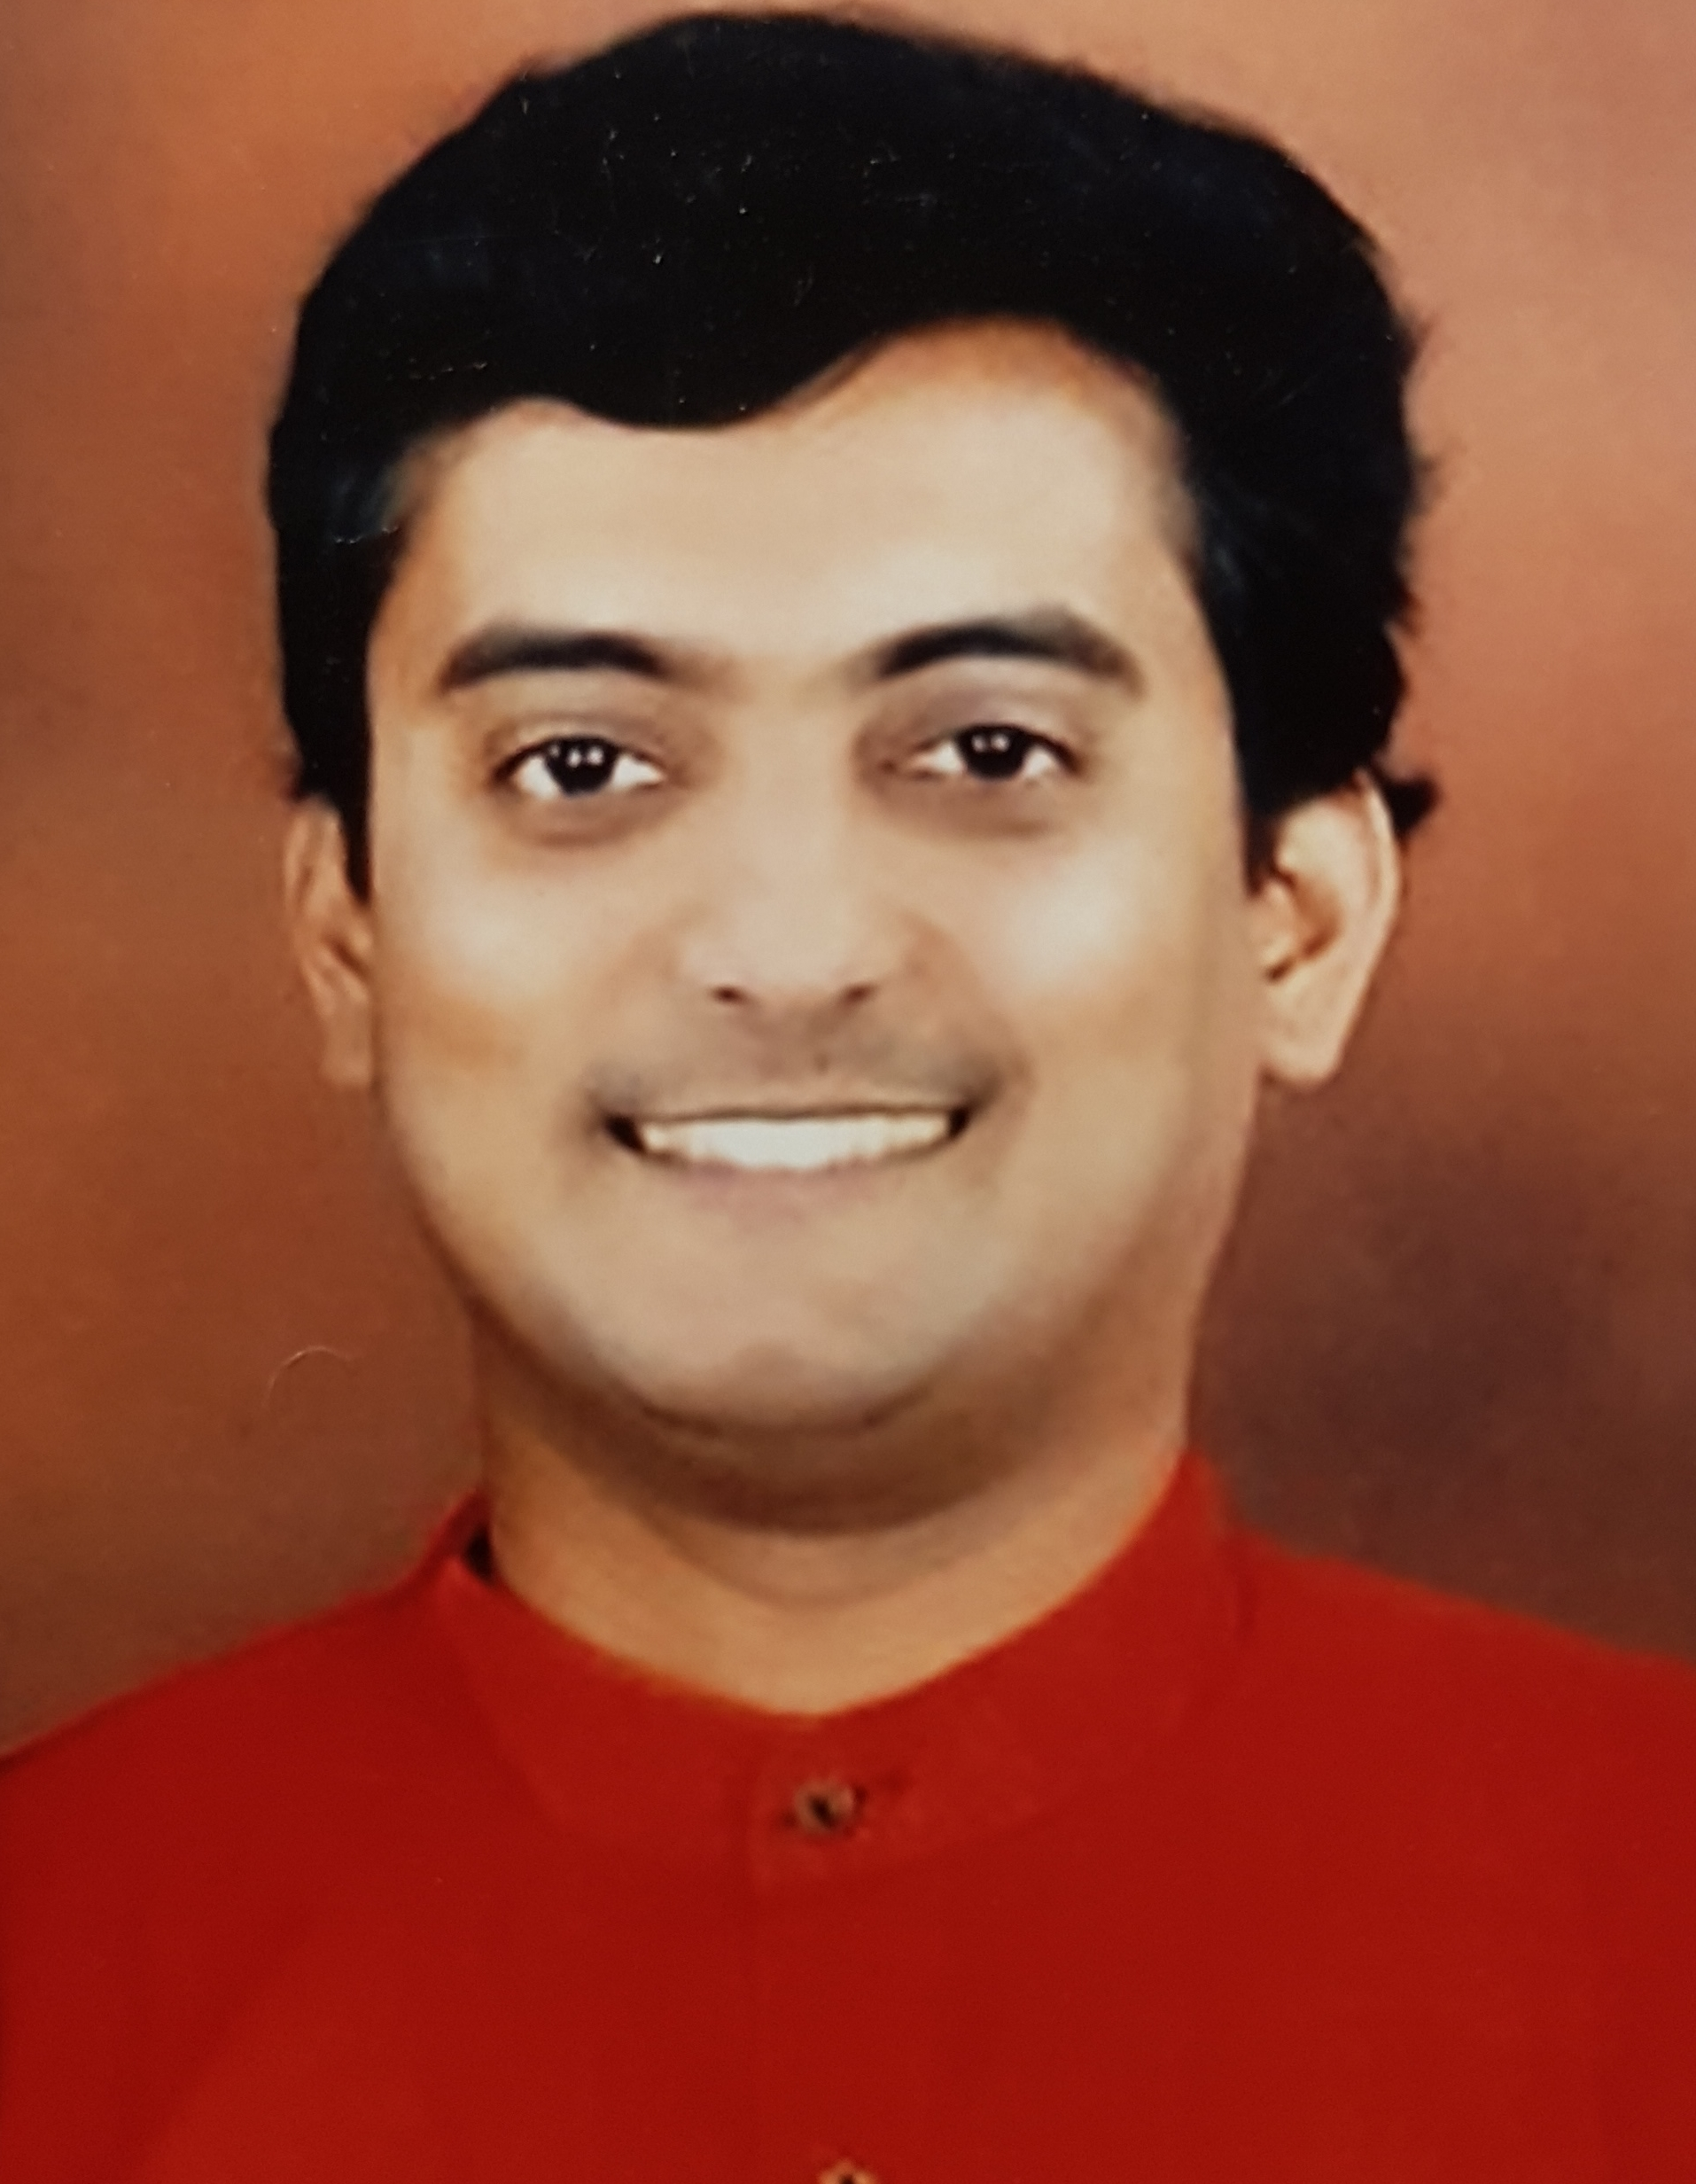
\includegraphics[scale=.18]{authorsphotos/Vinay_Deepak.eps}
\end{minipage}\quad
\begin{minipage}{6.5cm}
\textbf{Dr.\ Vinay Deepak} obtained the M.Sc.\ degree in 1999 from Bangalore University and Ph.D. in 2007 from Indian Institute of Science, Bangalore. After a year as Postdoctoral Researcher Fellow at the University of Southampton, he returned to the Physics Department, I.I.Sc. Bangalore, and worked there as a Research Associate from 2009 to 2010. He worked as an Assistant Professor at Jyoti Institute of Technology, Bangalore, from 2011 to 2014. From 2014 he has been working as Professor of Physics at BASE Educational Services Pvt.\ Ltd., Bangalore.
\end{minipage}

